\documentclass[10pt,twocolumn]{extarticle}
\usepackage[a4paper,margin=1.5cm,columnsep=0.7cm]{geometry}
\usepackage{amsmath,amssymb}
\usepackage{graphicx}
\usepackage{enumitem}
\usepackage{booktabs}
\usepackage{array}
\usepackage{tabularx}
\usepackage[T1]{fontenc}

\setlength{\parindent}{0pt}
\setlength{\parskip}{4pt}
\renewcommand{\arraystretch}{1.15}

\newenvironment{qoptions}{\begin{itemize}[leftmargin=1.8em,itemsep=2pt,topsep=2pt,label={}]}{\end{itemize}}
\newcommand{\opt}[2]{\item[({#1})] {#2}}

\newcommand{\sectionhdr}[1]{\par\vspace{4pt}\noindent\textbf{\large #1}\par\vspace{2pt}}
\newcommand{\subsectionhdr}[1]{\par\vspace{3pt}\noindent\textbf{#1}\par\vspace{2pt}}

\pagestyle{empty}

\begin{document}
\twocolumn[
\begin{center}
{\LARGE\bfseries JEE (Main+Advanced) Score-II --- Test 02 (28 Mar 2021)}
\end{center}
\vspace{6pt}
]

\sectionhdr{PAPER-1}

\sectionhdr{PART-1: PHYSICS}
\subsectionhdr{Section-I (i): Single Correct}

\textbf{1.} There is a system of 4 infinite length uniformly charged wires passing through corners of a rectangle ABCD and perpendicular to the plane of rectangle as shown in figure. Charge density of wires passing through A, D is $\lambda$ and B \& C is $2\lambda$. $P_1, P_2, P_3$ and $P_4$ are points on the perpendicular bisector of AD and BC.

\begin{center}
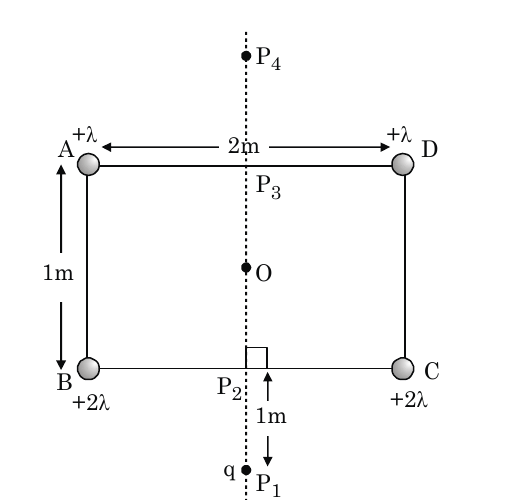
\includegraphics[width=0.9\linewidth]{Score-II - Test 02 (28 Mar 2021)-img/q1_rect.png}
\end{center}

\begin{qoptions}
\opt{A}{Potential energy of system is increasing continuously if a charge particle `q' is moved from $P_1$ to O along perpendicular bisectors.}
\opt{B}{Potential energy of system 1st increase then decrease if a charge particle `q' is moved from O to $P_3$}
\opt{C}{Potential energy of system decrease continuously if a charge particle `q' is moved from $P_2$ to O.}
\opt{D}{Potential energy of system 1st increase and then decrease if particle is moved from $P_2$ to O along perpendicular bisector line.}
\end{qoptions}

\textbf{2.} A light disc made of aluminium (a nonmagnetic material) is kept horizontally and is free to rotate about its axis as shown in the figure. A point charge particle is revolving about the axis of disc, then the disc will

\begin{center}
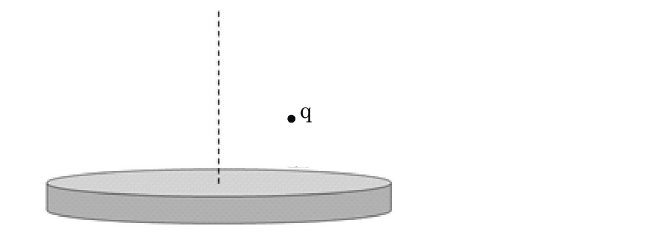
\includegraphics[width=0.75\linewidth]{Score-II - Test 02 (28 Mar 2021)-img/q2_disc.png}
\end{center}

\begin{qoptions}
\opt{A}{Rotate in the direction opposite to the direction of charge's motion.}
\opt{B}{Rotate in same direction as the direction of charge's motion.}
\opt{C}{Not rotate but temperature will increase.}
\opt{D}{Not rotate but its temperature will remain unchanged}
\end{qoptions}

\textbf{3.} An object is placed at distance 12 cm from top face of glass slab ($\mu=\sqrt2$). If the object is viewed from the position of observer as shown, then the apparent distance from the top surface of glass slab will be:

\begin{center}
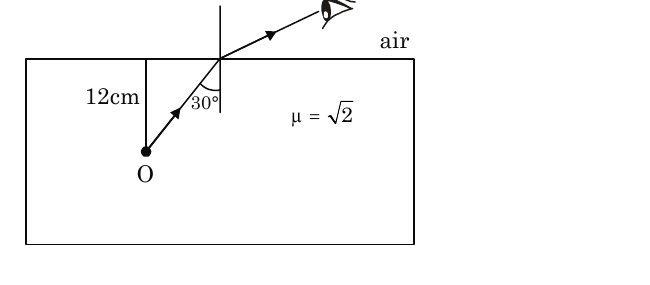
\includegraphics[width=0.75\linewidth]{Score-II - Test 02 (28 Mar 2021)-img/q3_slab.png}
\end{center}

\begin{qoptions}
\opt{A}{$\dfrac{4}{\sqrt3}$}
\opt{B}{$4\sqrt3$}
\opt{C}{$2\sqrt2$}
\opt{D}{$\dfrac{8}{\sqrt3}$}
\end{qoptions}

\textbf{4.} Smooth wire shaped as circular arc AC and CB are of same radius but centre of curvature are on opposite sides as shown. A small bead is projected horizontally from A with speed such that normal force become zero at point C. Speed of the particle when it reach to B will be [Take $\theta=\cos^{-1}(5/6)$]:

\begin{center}
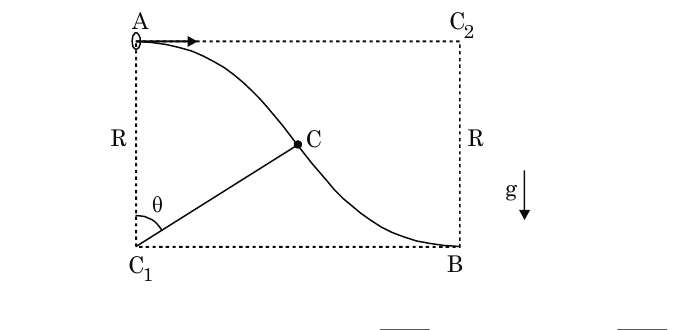
\includegraphics[width=0.85\linewidth]{Score-II - Test 02 (28 Mar 2021)-img/q4_arc.png}
\end{center}

\begin{qoptions}
\opt{A}{$\sqrt{2gR}$}
\opt{B}{$\sqrt{3gR}$}
\opt{C}{$\sqrt{\dfrac52gR}$}
\opt{D}{$\sqrt{\dfrac32gR}$}
\end{qoptions}

\subsectionhdr{Section-I (ii): One or more correct}

\textbf{5.} A boat start from point `P' from one bank of river with a sound siren of frequency $f$ move in the river in such a way that it crosses the river in minimum time. A detector is fixed at some height from the ground on the other bank just opposite to point P. If velocity of river flow is V, velocity of boat is $2V$ w.r.t. water flow and velocity of sound in air $=V_0$. Consider only sound pulse reach to detector only through air. Then [width of river $=d$ and $V\ll V_0$]

\begin{center}
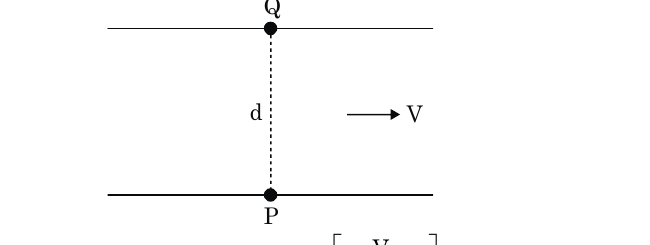
\includegraphics[width=0.75\linewidth]{Score-II - Test 02 (28 Mar 2021)-img/q5_river.png}
\end{center}

\begin{qoptions}
\opt{A}{Maximum frequency observed by detector $=\left[\dfrac{V_0}{V_0-2V}\right]f$}
\opt{B}{Maximum frequency observed by detector $=\left[\dfrac{V_0}{V_0-\sqrt3V}\right]f$}
\opt{C}{Detector will observed frequency $f$ when boat cross half of river.}
\opt{D}{Minimum frequency observed by detector $=\left[\dfrac{V_0}{V_0+3V}\right]f$}
\end{qoptions}

\textbf{6.} One end of a spring of negligible unstretched length and spring constant $k$ is fixed at the origin $(0,0)$. A point particle of mass $m$ carrying a positive charge $q$ is attached at its other end. The entire system is kept on a smooth horizontal surface. When some positive point charge `q' is fixed at the origin, the spring get stretched to a length $\ell$ and attains a new equilibrium position and at rest. If the spring is elongated slightly from equilibrium and released, it is found that

\begin{center}

\includegraphics[width=0.6\linewidth]{Score-II - Test 02 (28 Mar 2021)-img/q6_spring.png}
\end{center}

\begin{qoptions}
\opt{A}{Particle oscillate with time period $T=2\pi\sqrt{\dfrac{m}{3k}}$}
\opt{B}{Particle oscillate with time period $T=\pi\sqrt{\dfrac{m}{3k}}$}
\opt{C}{When particle move from mean position to extreme position then modulus of change in potential energy of spring is equal to modulus of change in electrostatic potential energy (for very small amplitude)}
\opt{D}{When particle move from mean position to extreme position then modulus of change in potential energy of spring is half modulus of change in electrostatic potential energy (for very small amplitude)}
\end{qoptions}

\textbf{7.} A uniform solid cone (height $h$, semi-vertex angle $\alpha$) is inclined against a vertical axis as shown in the figure. The cone rotates about its own axis as well as rotates about the vertical axis with angular speeds marked in the diagram. If the cone does not slip at point B, then

\begin{center}
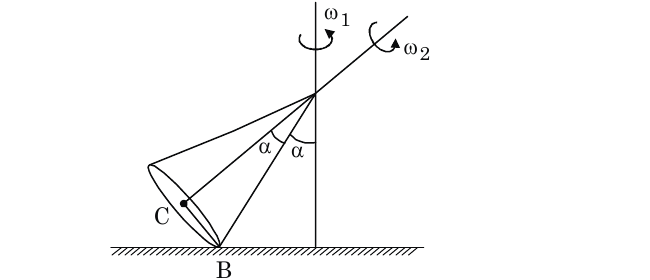
\includegraphics[width=0.85\linewidth]{Score-II - Test 02 (28 Mar 2021)-img/q7_cone.png}
\end{center}

\begin{qoptions}
\opt{A}{$\dfrac{\omega_1}{\omega_2}=1$}
\opt{B}{$\dfrac{\omega_1}{\omega_2}=\sqrt3$}
\opt{C}{Velocity of C $=h\sin2\alpha\,\omega_1$}
\opt{D}{Velocity of C $=h\omega_1$}
\end{qoptions}

\textbf{8.} A copper wire of density $\rho$ with cross-sectional area S bent to make three sides of a square can turn about a horizontal axis OO'. The wire is located in uniform vertical magnetic field. If on passing a current I through the wire the latter deflects by an angle $\theta$ and remain in equilibrium. Then

\begin{center}
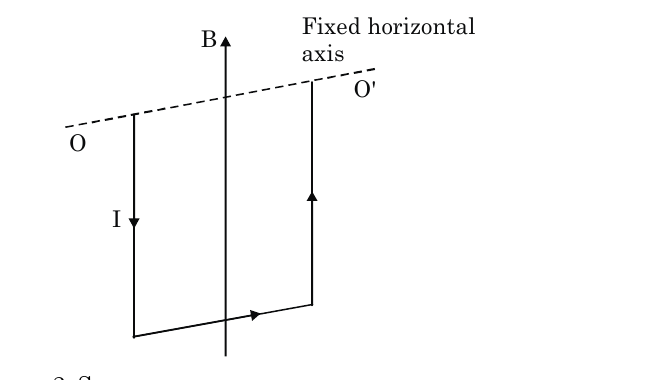
\includegraphics[width=0.85\linewidth]{Score-II - Test 02 (28 Mar 2021)-img/q8_wire.png}
\end{center}

\begin{qoptions}
\opt{A}{Magnetic field $B=\dfrac{2\rho Sg}{I}\tan\theta$}
\opt{B}{Magnetic field $B=\dfrac{2\rho Sg}{I}\sin\theta$}
\opt{C}{Net magnetic force on the copper wire is along horizontal.}
\opt{D}{Net magnetic force on the copper wire is zero.}
\end{qoptions}

\textbf{9.} Displacement (y) of air column of position x from its mean position at any instant is given by graph shown in the figure. We can conclude from graph that

\begin{center}
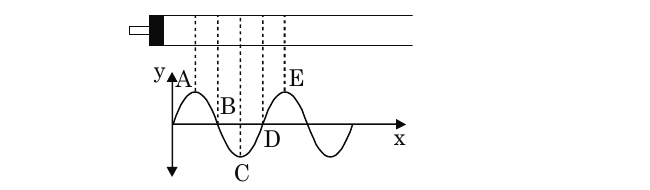
\includegraphics[width=0.85\linewidth]{Score-II - Test 02 (28 Mar 2021)-img/q9_graph.png}
\end{center}

\begin{qoptions}
\opt{A}{Average density in pipe is equal to density at point A at given instant}
\opt{B}{Average density in pipe is equal to density at point C at given instant}
\opt{C}{Density of air is maximum at B}
\opt{D}{Density of air is minimum at D}
\end{qoptions}

\textbf{10.} A proton collides with a stationary deuteron and a $^3$He nucleus is formed. For this reaction to take place, the proton must have minimum kinetic energy 1.4 MeV. If instead, a deuteron collides with a stationary proton to make a $^3$He nucleus. Then

\begin{qoptions}
\opt{A}{minimum kinetic energy deuteron must possess $=2.8$ MeV}
\opt{B}{minimum kinetic energy deuteron must possess $=0.7$ MeV}
\opt{C}{Energy needed for the reaction is approx 0.93 MeV}
\opt{D}{Energy needed for the reaction is approx 2.8 MeV}
\end{qoptions}

\textbf{11.} Two large circular discs separated by a distance of 0.01 m are connected to a battery via switch as shown in the figure. Charged oil drops of density 900 kg/m$^3$ are released through a tiny hole at the centre of the top disc. Once some oil drops achieve terminal velocity, the switch is closed to apply a voltage of 200 V across the disc and also an external electric field $E=4\times10^4$ along vertically downwards is applied. As a result, an oil drop of radius $8\times10^{-7}$ m stops moving vertically and floats between the discs. (Neglect the buoyancy force, take acceleration due to gravity $=10$ m/s$^2$ and $e=1.6\times10^{-19}$ C]

\begin{center}
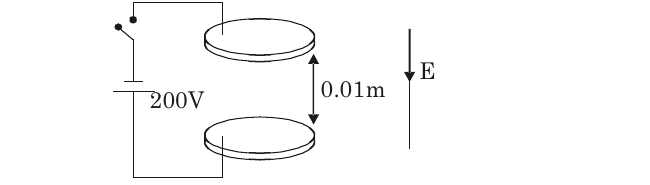
\includegraphics[width=0.85\linewidth]{Score-II - Test 02 (28 Mar 2021)-img/q11_discs.png}
\end{center}

\begin{qoptions}
\opt{A}{The number of electrons present in this oil drop is 6.}
\opt{B}{The number of electrons present in this oil drop is 18.}
\opt{C}{Net electric field between disc is $2\times10^4$ V/m}
\opt{D}{Net electric field between disc is $6\times10^4$ V/m}
\end{qoptions}

\textbf{12.} In the balanced condition, the values of the resistances of the four arms of a wheatstone bridge are shown in figure below. The resistance $R_3$ has temperature coefficient $\alpha=KT\,^\circ\text{C}^{-1}$ where $K=0.0008$ and $T$ is in $^\circ$C. If the temperature of only $R_3$ is increased by $10^\circ$C, then [Take initial temperature $0^\circ$C; Resistance of voltmeter V is very large]

\begin{center}
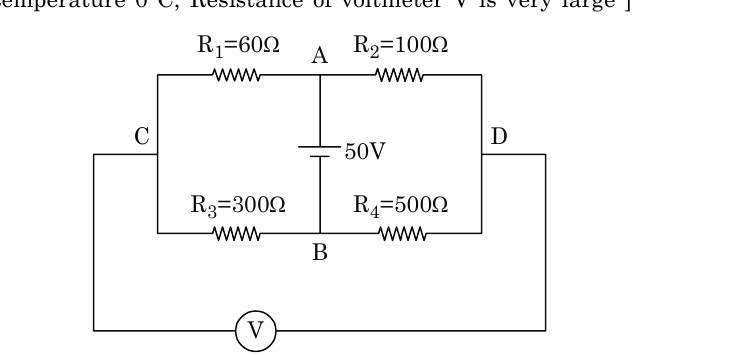
\includegraphics[width=0.95\linewidth]{Score-II - Test 02 (28 Mar 2021)-img/q12_bridge.png}
\end{center}

\begin{qoptions}
\opt{A}{the voltage developed between C and D will be approx 0.27 volt at $T=10^\circ$C}
\opt{B}{the voltage developed between C and D will be approx 0.47 volt at $T=10^\circ$C}
\opt{C}{the voltage developed between C and D will be 0 volt at $T=0^\circ$C}
\opt{D}{the voltage developed between C and D will be 0.5 volt at $T=0^\circ$C}
\end{qoptions}

\subsectionhdr{Section-II: Numerical Value}

\textbf{1.} An initially uncharged capacitor and inductor are connected to battery at $t=0$. Find the maximum energy stored in the inductor in Joule? [Take $C=1$F, $L=1$H and $E=5$V]

\begin{center}
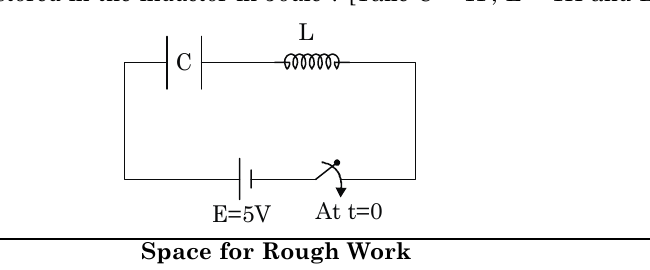
\includegraphics[width=0.7\linewidth]{Score-II - Test 02 (28 Mar 2021)-img/n1_lc.png}
\end{center}

\textbf{2.} A cylindrical pipe (no base) of radius R and mass M is placed vertically on a horizontal floor. Two identical spheres each of radius $\dfrac{3R}{4}$ and mass m are inserted in the cylinder as shown in the figure. At what minimum value of $m/M$ will the arrangement topple? There is no friction between the spheres and inner wall of the cylinder.

\begin{center}
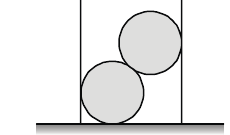
\includegraphics[width=0.55\linewidth]{Score-II - Test 02 (28 Mar 2021)-img/n2_cyl.png}
\end{center}

\textbf{3.} Two elastic balls of masses $m_1$ and $m_2$ are placed on top of each other (with a small gap between them) and then dropped onto the ground. What is the ratio $m_2/m_1$, for which the upper ball ultimately receives the largest possible fraction of the total energy?

\textbf{4.} Consider a quarter circular conducting ring of large radius $r$ with its centre at the origin, where a small magnetic dipole of dipole moment $\vec m$ is placed as shown in the figure. If the ring rotates at a constant angular velocity $\omega$ about the y-axis, and electromotive force induced between its ends is $p\dfrac{\mu_0m\omega}{\pi r}$. Find $p$.

[\textbf{Note:} Write magnetic field due to small magnetic dipole in the same way as due to electric dipole]

\begin{center}
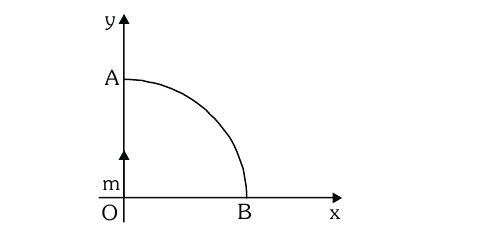
\includegraphics[width=0.55\linewidth]{Score-II - Test 02 (28 Mar 2021)-img/n4_ring.png}
\end{center}

\textbf{5.} Wedge A with block B of mass $m$ placed on it get a horizontal acceleration `a' directed to the left at shown in figure. Friction coefficient between block and inclined surface $\mu=\dfrac{1}{2\sqrt3}$. Find the minimum value of the acceleration (in m/s$^2$) so that the block will remain stationary w.r.t. wedge (Take: $g=10$ m/s$^2$)

\begin{center}
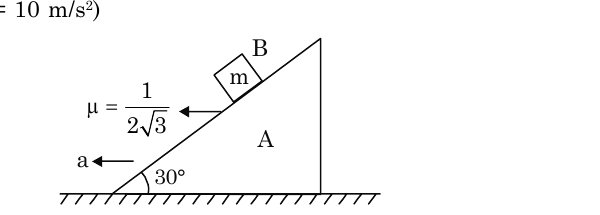
\includegraphics[width=0.75\linewidth]{Score-II - Test 02 (28 Mar 2021)-img/n5_wedge.png}
\end{center}

\textbf{6.} A small bead can slide without friction on a wooden rod of length $\ell=10.0$ m. Initially the rod and the bead both are held motionless with the rod aligned radially with the earth. The left end of the rod is at a distance $r_0=4\times10^8$ m from the earth centre and the bead is at a distance $x_0=2.0$ cm away from the left end. Both the bodies are released simultaneously. Considering gravitational interaction only with the earth, if time after the release, the bead will separate from the rod is $P\times10^4$ sec. Find P. Radius of the earth is $R=6400$ km and acceleration due to gravity on the earth is $g=10$ m/s$^2$.

\begin{center}
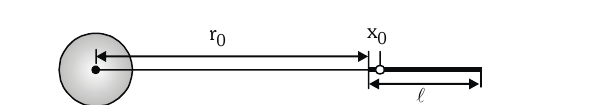
\includegraphics[width=0.85\linewidth]{Score-II - Test 02 (28 Mar 2021)-img/n6_rod.png}
\end{center}

\sectionhdr{PART-2: CHEMISTRY}
\subsectionhdr{Section-I (i): Single Correct}

\textbf{1.} The molar conductance of H$^+$ ion and CH$_3$COO$^-$ ion at 298K and at infinite dilution are $3.474\times10^{-2}\,\Omega^{-1}\text{m}^2\text{mol}^{-1}$ and $1.351\times10^{-2}\,\Omega^{-1}\text{m}^2\text{mol}^{-1}$, respectively. The resistance of 0.1 M CH$_3$COOH solution is 2000 ohm at 298K in a conductivity cell of cell constant 20 m$^{-1}$. The incorrect information related with the given parameters at 298K is (1F $=$ 96500 C/mol)

\begin{qoptions}
\opt{A}{$\Lambda_m^0(\text{CH}_3\text{COOH})=4.825\times10^{-2}\,\Omega^{-1}\text{m}^2\text{mol}^{-1}$}
\opt{B}{$\kappa=1.0\times10^{-2}\,\Omega^{-1}\text{m}^{-1}$}
\opt{C}{$\Lambda_m=1.0\times10^{-4}\,\Omega^{-1}\text{m}^2\text{mol}^{-1}$}
\opt{D}{$[\text{H}^+]=2.07\times10^{-3}$ M}
\end{qoptions}

\textbf{2.} If $n$ and $l$ are the principal and Azimuthal quantum numbers respectively, then the expression for calculating the maximum number of electrons in any orbit is

\begin{qoptions}
\opt{A}{$\displaystyle\sum_{l=1}^{l=n}2(2l+1)$}
\opt{B}{$\displaystyle\sum_{l=1}^{l=n-1}2(2l+1)$}
\opt{C}{$\displaystyle\sum_{l=0}^{l=n+1}2(2l+1)$}
\opt{D}{$\displaystyle\sum_{l=0}^{l=n-1}2(2l+1)$}
\end{qoptions}

\textbf{3.} Select incorrect statement(s) w.r.t these 4 species.

\begin{center}
\renewcommand{\arraystretch}{1}
\begin{tabular}{@{}cc@{}}
(I)\;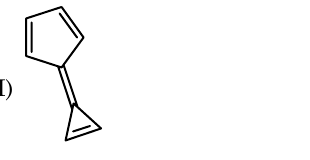
\includegraphics[width=2.6cm]{Score-II - Test 02 (28 Mar 2021)-img/q3_I.png} &
(II)\;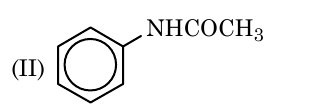
\includegraphics[width=3.0cm]{Score-II - Test 02 (28 Mar 2021)-img/q3_II.png} \\[6pt]
(III)\;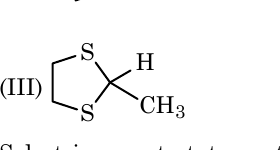
\includegraphics[width=2.6cm]{Score-II - Test 02 (28 Mar 2021)-img/q3_III.png} &
(IV)\;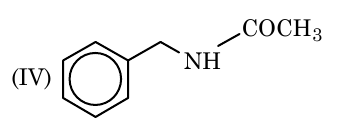
\includegraphics[width=3.0cm]{Score-II - Test 02 (28 Mar 2021)-img/q3_IV.png} \\
\end{tabular}
\renewcommand{\arraystretch}{1.15}
\end{center}

\begin{qoptions}
\opt{A}{I is polar hydrocarbon}
\opt{B}{II is more acidic than aniline}
\opt{C}{III is more acidic than acetal formed by ethanal \& ethylene glycol}
\opt{D}{IV is less basic than II.}
\end{qoptions}

\textbf{4.} \textbf{Statement-I:} On increasing the temperature of an elementary biomolecular gaseous reaction by $10^\circ$C occuring at constant volume, the rate of reaction increase substantially by factor of 2 to 3.

\textbf{Statement-2:} The increase in temperature increases the collision frequency (total number of biomolecular collisions per unit time per unit volume) for the above condition.

\begin{qoptions}
\opt{A}{Statement-1 is true, Statement-2 is true and statement-2 is correct explanation for statement-1.}
\opt{B}{Statement-1 is true, Statement-2 is true and statement-2 is NOT correct explanation for statement-1.}
\opt{C}{Statement-1 is true, statement-2 is false.}
\opt{D}{Statement-1 is false, statement-2 is true.}
\end{qoptions}

\subsectionhdr{Section-I (ii): One or more correct}

\textbf{5.} Among the following INCORRECT with reference to MOT is/are.

\begin{center}
\begin{tabular}{@{}ll@{}}
\multicolumn{2}{@{}l}{\textbf{Orbital overlapped} \hspace{2.5cm}\textbf{Properties}}\\[4pt]
\end{tabular}
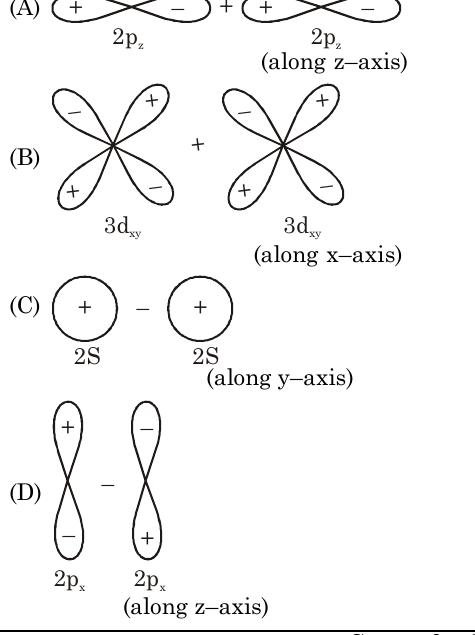
\includegraphics[width=0.72\linewidth]{Score-II - Test 02 (28 Mar 2021)-img/q5_all.png}
\end{center}

\begin{qoptions}
\opt{A}{Orbital overlap of $2p_z+2p_z$ (along z-axis) $\to$ Gerade, LUMO of C$_2$}
\opt{B}{Orbital overlap of $3d_{xy}+3d_{xy}$ (along x-axis) $\to$ Gerade, $\sigma$-bond is formed}
\opt{C}{Orbital overlap of $2S-2S$ (along y-axis) $\to$ Ungerade, HOMO of Li$_2$}
\opt{D}{Orbital overlap of $2p_x-2p_x$ (along z-axis) $\to$ Ungerade, HOMO of B$_2$}
\end{qoptions}

\textbf{6.} Which of the following reaction is/are correct?

\begin{center}
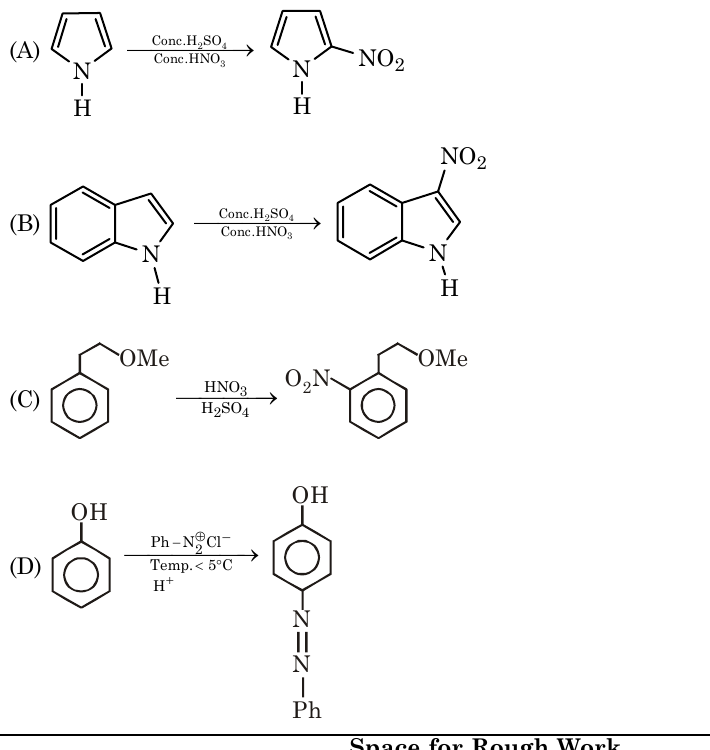
\includegraphics[width=0.85\linewidth]{Score-II - Test 02 (28 Mar 2021)-img/q6_all.png}
\end{center}

\begin{qoptions}
\opt{A}{Pyrrole $\xrightarrow[\text{Conc.HNO}_3]{\text{Conc.H}_2\text{SO}_4}$ 2-nitropyrrole (as shown)}
\opt{B}{Indole $\xrightarrow[\text{Conc.HNO}_3]{\text{Conc.H}_2\text{SO}_4}$ 3-nitroindole (as shown)}
\opt{C}{2-methoxyethylbenzene $\xrightarrow[\text{H}_2\text{SO}_4]{\text{HNO}_3}$ ortho-nitro product (as shown)}
\opt{D}{Phenol $\xrightarrow[\text{H}^+]{\text{Ph-N}_2^+\text{Cl}^-,\ T<5^\circ\text{C}}$ para-azo coupled product (as shown)}
\end{qoptions}

\textbf{7.} Which of the following statements is/are incorrect w.r.t enzyme catalysed reactions.

\begin{qoptions}
\opt{A}{The cavities on enzyme ``Maltase'' \& structure of molecules of Maltose have complimentary shapes for conversion of Maltase to glucose.}
\opt{B}{Just like other catalysts, catalytic action of enzyme is more at a lower temperature.}
\opt{C}{In presence of vitamins \& metal ions; enzyme activity generally increases.}
\opt{D}{Most of the enzyme catalysed reactions are elementary.}
\end{qoptions}

\textbf{8.} Which of the following option(s) represent the INCORRECT IUPAC name of the given co-ordination compounds?

\begin{qoptions}
\opt{A}{Li[CuMe$_2$] : Lithium dimethylcuprate(II).}
\opt{B}{[Os(Et)(NH$_3)_5$]Cl : Pentaammineethylosmium(II) chloride.}
\opt{C}{K$_3$[Co(CN)$_5$H] : Potassium pentacyanidoprotoniumcobaltate(I)}
\opt{D}{[Co(en)$_3$]Cl$_3$ : Tris-(ethane-1,2-diammine)cobalt(III) chloride.}
\end{qoptions}

\textbf{9.} Select correct options.

\begin{qoptions}
\opt{A}{Meso tartaric acid is aldaric acid of L-erythrose}
\opt{B}{D-Mannose \& D-Galactose form same osazone}
\opt{C}{D-Mannose \& D-Galactose are epimers}
\opt{D}{All monosaccharides are reducing sugars}
\end{qoptions}

\textbf{10.} Identify correct option(s) among following statements -

\begin{qoptions}
\opt{A}{In Na$_2$O crystal oxide ion is present in a cubic void formed by Na$^+$ ions}
\opt{B}{AgBr shows both schottky and frenkel defects}
\opt{C}{Metals can conduct electricity in molten state}
\opt{D}{Fe$_{0.95}$O crystal can work as n-type semiconductor.}
\end{qoptions}

\textbf{11.} Select CORRECT ``statement \& reason'' combinations

\begin{center}
\renewcommand{\arraystretch}{1.2}
\begin{tabular}{@{}p{4.0cm}p{3.6cm}@{}}
\textbf{Statement} & \textbf{Correct reason} \\
(A) Argentite ore is concentrated by froth floatation process. & Argentite is a sulphide ore. \\[4pt]
(B) During calcination, the ore is heated well below its melting point in the limited supply of oxygen. & The process of calcination is carried out for sulphide ores only. \\[4pt]
(C) Highly electropositive metals are extracted by electrolysis of their aq. salt solutions. & Highly electropositive metals cannot be reduced by chemical reduction using Carbon \\[4pt]
(D) The process involved in the extraction of tin from tin stone is the carbon reduction. & Reduction of cassiterite to metal by carbon is feasible at convenient temperature. \\
\end{tabular}
\renewcommand{\arraystretch}{1.15}
\end{center}

\textbf{12.} Select the incorrect options:

\begin{center}
(A)\; \raisebox{-0.4\height}{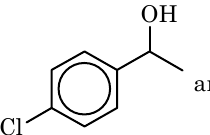
\includegraphics[width=2.0cm]{Score-II - Test 02 (28 Mar 2021)-img/q12_A1.png}} \; and \; \raisebox{-0.4\height}{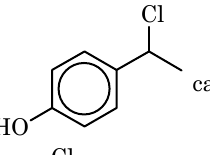
\includegraphics[width=2.0cm]{Score-II - Test 02 (28 Mar 2021)-img/q12_A2.png}} \; can be differentiated by 2,4-DNP test.

\vspace{4pt}
(B)\; \raisebox{-0.4\height}{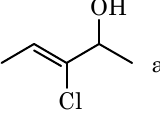
\includegraphics[width=1.5cm]{Score-II - Test 02 (28 Mar 2021)-img/q12_B1.png}} \; and \; \raisebox{-0.4\height}{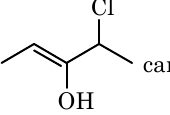
\includegraphics[width=1.5cm]{Score-II - Test 02 (28 Mar 2021)-img/q12_B2.png}} \; can be differentiated by NaHCO$_3$ test.

\vspace{4pt}
(C)\; \raisebox{-0.4\height}{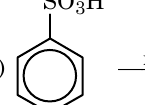
\includegraphics[width=1.7cm]{Score-II - Test 02 (28 Mar 2021)-img/q12_C.png}} $\xrightarrow[\text{Fuse}]{\text{NaOH}}$ Product give violet colour with neutral FeCl$_3$

\vspace{4pt}
(D) With NaOI, \; \raisebox{-0.4\height}{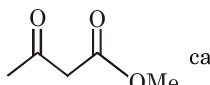
\includegraphics[width=2.6cm]{Score-II - Test 02 (28 Mar 2021)-img/q12_D.png}} \; can give yellow ppt.
\end{center}

\subsectionhdr{Section-II: Numerical Value}

\textbf{1.} N$_2$(g) $+$ 3H$_2$(g) $\rightleftharpoons$ 2NH$_3$(g), $\Delta G^0_{f(\text{NH}_3)}=-15.53$ kJ/mole at 300 K. If after 1 hour of mixing reactants, partial pressure of N$_2=50$ Bar, H$_2=2$ Bar, NH$_3=200$ Bar \& $\Delta H_{\text{reaction}}$ is $-4.2$ kJ, find $\Delta S$ of reaction (in JK$^{-1}$). ($\ln10=2.3$, $R=\dfrac{25}{3}$ JK$^{-1}$mol$^{-1}$).

\textbf{2.} A solution of white crystals gives a precipitate with AgNO$_3$ but no precipitation with a solution of Na$_2$CO$_3$. The action of concentrated H$_2$SO$_4$ on the crystals yields coloured fumes. Find the number of crystals given below which can give above observation:\\
NaI, KCl, NaNO$_2$, NaBr, CH$_3$COONa

\textbf{3.} An aldehyde (A) (C$_{11}$H$_8$O), which does not undergo self Aldol condensation, gives benzaldehyde and two moles of (B) on reductive ozonolysis. Compound (B) on oxidation with silver ion gives oxalic acid. (A) on reduction with Lindlar's catalyst produces (C), which reduces Tollen's reagent. How many geometrical isomers (C) can exhibit?

\textbf{4.} The uncertainty in the position of an electron is equal to its de-Broglie wavelength. Find the minimum percentage error in measurement of its velocity under this circumstance.

\textbf{5.} How many of the following reactions produce H$_2$ gas as (one of the) product.

\begin{center}
\renewcommand{\arraystretch}{1.3}
\begin{tabular}{@{}p{0.46\linewidth}p{0.46\linewidth}@{}}
(i) HI $\xrightarrow{\Delta}$ & (ii) C $+$ H$_2$O $\xrightarrow{1300\text{K}}$ \\
(iii) Zn $+$ NaOH$_{(aq.)}\longrightarrow$ & (iv) CH$_4+$H$_2$O $\xrightarrow{1000^\circ\text{C}}$ \\
(v) NaOH$_{(aq)}+$Al$+$H$_2$O$\longrightarrow$ & (vi) LiH$+$B$_2$H$_6\longrightarrow$ \\
(vii) SiCl$_4+$H$_2$O$\longrightarrow$ & (viii) NaH$+$CH$_3$COOH$\longrightarrow$ \\
(ix) NaH$_{(\text{molten})}\xrightarrow{\text{electrolysis}}$ & (x) NaCl$_{(\text{molten})}\xrightarrow{\text{electrolysis}}$ \\
\end{tabular}
\renewcommand{\arraystretch}{1.15}
\end{center}

\textbf{6.} For the compound shown below:

\begin{center}
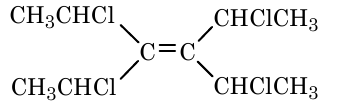
\includegraphics[width=0.75\linewidth]{Score-II - Test 02 (28 Mar 2021)-img/n6_alkene.png}
\end{center}

For above compound's\\
P $\to$ total number of stereoisomers.\\
Q $\to$ total number of enantiomeric pairs\\
R $\to$ total number of meso compounds\\
Then give your answer in 3 digit's as PQR

\sectionhdr{PART-3: MATHEMATICS}
\subsectionhdr{Section-I (i): Single Correct}

\textbf{1.} Suppose a, b denote the distinct real root of the quadratic polynomial $x^2+5x-100=0$ and suppose c, d denote the distinct complex root of the polynomial $x^2-5x+100=0$, then the value of $ac(a^2+c^2)+bc(b^2+c^2)+ad(a^2+d^2)+bd(b^2+d^2)$ is

\begin{qoptions}
\opt{A}{0}
\opt{B}{$-1250$}
\opt{C}{15000}
\opt{D}{8125}
\end{qoptions}

\textbf{2.} If the function $f:\mathbb{R}\to\mathbb{R}$, $f(x)=-\left(\sqrt{x^2}\sin x-x\sqrt{x^2}\right)$, then which of following statement is true?

\begin{qoptions}
\opt{A}{f is one-one but not onto}
\opt{B}{f is one-one and onto}
\opt{C}{f is many one and onto}
\opt{D}{f is neither one-one nor onto}
\end{qoptions}

\textbf{3.} Let the function $f:\mathbb{R}\to\mathbb{R}$ and $g:\mathbb{R}\to\mathbb{R}$ be defined by $f(x)=e^x-e^{-|x|}$ and $g(x)=\dfrac{e^x+e^{-x}}{3}$ then the area bounded by the curves $y=f(x)$, $y=g(x)$ and $x=0$ in the first quadrant is

\begin{qoptions}
\opt{A}{$\dfrac{6\sqrt2}{3}-2$}
\opt{B}{$\dfrac{4\sqrt2}{3}+2$}
\opt{C}{$\dfrac{6\sqrt2}{3}+2$}
\opt{D}{$2-\dfrac{4\sqrt2}{3}$}
\end{qoptions}

\textbf{4.} For the ellipse $\dfrac{x^2}{9}+\dfrac{y^2}{4}=1$ with vertices A(3,0) and A$'(-3,0)$, tangent drawn at the point P in the I quadrant meets the y-axis at Q and the chord A$'$P meet the y-axis at M. If O is the origin, then $OQ^2-MQ^2$ equals to

\begin{qoptions}
\opt{A}{9}
\opt{B}{13}
\opt{C}{4}
\opt{D}{5}
\end{qoptions}

\subsectionhdr{Section-I (ii): One or more correct}

\textbf{5.} The probability of a man hitting a target in one fire is $\dfrac15$. If N denotes the minimum number of fire required to make his chances of hitting a target more than $\dfrac34$, then N$+2$ is

\begin{qoptions}
\opt{A}{Odd number}
\opt{B}{Perfect square}
\opt{C}{Even number}
\opt{D}{Prime number}
\end{qoptions}

\textbf{6.} Let $f(x)=\sin^2x-\sin x+2$, $x\in(0,\pi)$. Suppose f has local minimum at $x=\{k_1\pi,k_2\pi,\ldots,k_n\pi\}$ where $0<k_1<k_2<k_3<\cdots<k_n<1$. If $N=k_1+k_2+\cdots+k_n$, then which following options are incorrect.

\begin{qoptions}
\opt{A}{N is prime number}
\opt{B}{N is composite number}
\opt{C}{N is odd number}
\opt{D}{N is even number}
\end{qoptions}

\textbf{7.} Let `f' be a differentiable function satisfying $f(x+y)=f(x)+f(y)+(e^x-1)(e^y-1)$ $\forall\, x,y\in\mathbb{R}$ and $f'(0)=2$. Identify the correct statement(s)

\begin{qoptions}
\opt{A}{$\displaystyle\lim_{x\to0}\dfrac{f(f(x))}{f(x)-x}=4$}
\opt{B}{$\displaystyle\lim_{x\to0}\left(f(x)+\cos x\right)^{\frac{1}{e^x-1}}=e^2$}
\opt{C}{Number of solutions of the equation $f(x)=0$ is 2.}
\opt{D}{Range of the function $y=f(x)$ is $(-\infty,\infty)$.}
\end{qoptions}

\textbf{8.} If $A=\begin{pmatrix}u&2&-1\\-1&1&2\\2&-1&1\end{pmatrix}$, where $u\ne-\dfrac{11}{3}$ and $\det(\operatorname{adj}(\operatorname{adj}A))=23^4$ then which of the following options can be TRUE?

\begin{qoptions}
\opt{A}{$|A|=23$}
\opt{B}{$|A|=-\sqrt{23}$}
\opt{C}{$u=4$}
\opt{D}{$u=-4$}
\end{qoptions}

\textbf{9.} Let A be a subset of the real numbers such that $A=\{a\mid a=|z^2+z-1|\}$ in which z is a complex number such that $|z|=1$, then

\begin{qoptions}
\opt{A}{Maximum possible value of a is 5}
\opt{B}{Maximum possible value of a is $\sqrt5$}
\opt{C}{Minimum possible value of a is 1}
\opt{D}{Minimum possible value of a is $\sqrt2$}
\end{qoptions}

\textbf{10.} Suppose x, y, z are the length of side of a triangle opposite to it angles X, Y and Z respectively if
\[\tan X+\tan Y=\dfrac{-2}{\sqrt3},\quad \tan Y+\tan Z=\dfrac{2}{\sqrt3}\ \text{and}\ x=2\sqrt3\]
then which of the following statement is/are true?

\begin{qoptions}
\opt{A}{X = Y + Z}
\opt{B}{X = 2(Y + Z)}
\opt{C}{$\tan\dfrac{X}{2}=\dfrac{2x}{y+z}$}
\opt{D}{In radius of $\triangle XYZ$ is $\dfrac{\sqrt3}{\left(2+\sqrt3\right)}$}
\end{qoptions}

\textbf{11.} (1, 0, $-1$) is the image of point (p, q, r) w.r.t. plane $x+y=3$. Then which of the following statements is/are true.

\begin{qoptions}
\opt{A}{$|p|+|q|+|r|=6$}
\opt{B}{$p+q+5r=0$}
\opt{C}{$p-q+r=0$}
\opt{D}{$p=2$}
\end{qoptions}

\textbf{12.} Which of the following is/are true

\begin{qoptions}
\opt{A}{$\displaystyle\int_0^1 x\tan x\,dx\ge\dfrac25$}
\opt{B}{$\displaystyle\int_0^1 x^2\tan x\,dx\le\dfrac{11}{36}$}
\opt{C}{$\displaystyle\int_0^1 x^2\tan x\,dx\ge\dfrac{11}{36}$}
\opt{D}{$\displaystyle\int_0^1 x\tan x\,dx\le\dfrac25$}
\end{qoptions}

\subsectionhdr{Section-II: Numerical Value}

\textbf{1.} Let N be the maximum value of $(\log_4p_1+\log_4p_2+\log_4p_3+\log_4p_4)$ where $p_1,p_2,p_3,p_4\in\mathbb{R}^+$. Also $p_1+p_2+p_3+p_4=16$. Find the value of $\log_2N^2$.

\textbf{2.} If $\{x_n\}$ is a sequence of numbers $\forall\, n\in\mathbb{N}$ such that
\[x_{n+1}=\dfrac{x_n+x_n^2}{1+x_n+x_n^2}\ \&\ x_1=\dfrac12\]
and $\displaystyle N=\dfrac{1}{x_1+1}+\dfrac{1}{x_2+1}+\cdots+\dfrac{1}{x_{2012}+1}+\dfrac{1}{x_{2013}}$.
Then sum of digits of N is equal to

\textbf{3.} Find the number of solutions of $\theta$ in $(0,2\pi)$ that satisfy the equation
\[\dfrac{1}{\sin^2\theta}-\dfrac{1}{\cos^2\theta}-\dfrac{1}{\tan^2\theta}-\dfrac{1}{\cot^2\theta}-\dfrac{1}{\sec^2\theta}-\dfrac{1}{\operatorname{cosec}^2\theta}=-3\]

\textbf{4.} In a $\triangle ABC$, AB $=4$, AC $=5$, O is circumcenter of $\triangle ABC$. Find the value of $2\overrightarrow{AO}\cdot\overrightarrow{BC}$?

\textbf{5.} For a polynomial $g(x)$ with real coefficient, let $m_g$ denote the number of distinct real roots of $g(x)$. Suppose S is the set of polynomials with real coefficients defined by
\[\resizebox{0.95\linewidth}{!}{$S=\left\{(x^2-1)^4(a_0+2a_1x+3a_2x^2+4a_3x^3):a_0,a_1,a_2,a_3\in\mathbb{R}\right\}$}\]
For a polynomial f, let $f'$ and $f''$ denote the first and second derivative of f then minimum possible value of $m_{f'}+m_{f''}$ where $f\in S$ is

\textbf{6.} The value of limit
\[\lim_{x\to0}\dfrac{\sin(3x+a)-3\sin(2x+a)+3\sin(x+a)-\sin a}{x^3}\]
is $-\cos\left(\dfrac{3a}{\lambda}\right)$. Then value of $\lambda$ is (where $\lambda\in\mathbb{N}$)

\sectionhdr{PAPER-2}

\sectionhdr{PART-1: PHYSICS}
\subsectionhdr{Section-I (i): One or more correct}

\textbf{1.} A small dipole of dipole moment $\vec P_2$ of mass m is suspended vertically by a string of length $\ell$. A small dipole of dipole moment $\vec P_1$ is now brought towards $\vec P_2$ from infinity so that the $P_2$ moves away and gravitational potential energy of dipole $P_1$ does not change. The final equilibrium position of the system including the direction of dipole, the angles and distance is shown in figure (where g is the acceleration due to gravity). Choose the correct statement(s):

\begin{center}
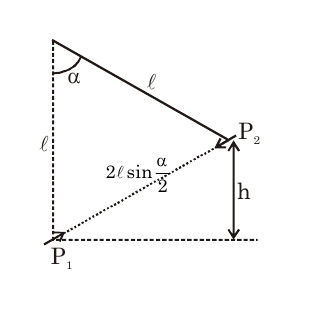
\includegraphics[width=0.42\linewidth]{Score-II - Test 02 (28 Mar 2021)-img/p2phy_q1_dipole.png}
\end{center}

\begin{qoptions}
\opt{A}{The work done in bringing the dipole to this position is $\dfrac{4mgh}{3}$}
\opt{B}{The work done in bringing the dipole to this position is $\dfrac{5mgh}{3}$}
\opt{C}{Change in electrostatic potential energy of dipole is $\dfrac{mgh}{3}$}
\opt{D}{Change in electrostatic potential energy of dipole is $\dfrac{2mgh}{3}$}
\end{qoptions}

\textbf{2.} A triangular rod frame ABC having equal mass `M' of all three sides. Rod AB and BC are of length $=$ L. Then the moment of inertia of triangular frame about:

\begin{center}
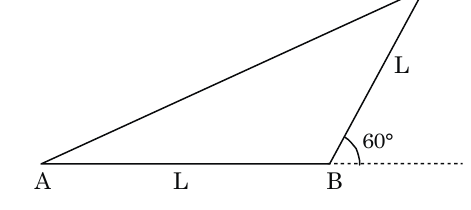
\includegraphics[width=0.62\linewidth]{Score-II - Test 02 (28 Mar 2021)-img/p2phy_q2_triangle.png}
\end{center}

\begin{qoptions}
\opt{A}{An axis perpendicular to AB and passing through B and in the plane of triangle is $\dfrac23 M\ell^2$}
\opt{B}{An axis perpendicular to AB and passing through B and in the plane of triangle is $\dfrac34 M\ell^2$}
\opt{C}{An axis perpendicular to AB and passing through A and in the plane of triangle is $\dfrac83 M\ell^2$}
\opt{D}{An axis perpendicular to AB and passing through A and in the plane of triangle is $\dfrac{10}{3} M\ell^2$}
\end{qoptions}

\textbf{3.} The filament of a light bulb has surface area 64 mm$^2$. The filament can be considered as a black body at temperature 2500 K emitting radiation like a point source. At night the light bulb is observed from a distance of 10 m. Assume light detector to be circular with radius $r=10\sqrt3$ m. Then (Take $\sigma=5.67\times10^{-8}$ Wm$^{-2}$K$^4$, Wien's displacement constant $=2.90\times10^{-3}$ m-K, Planck's constant $=6.63\times10^{-34}$ Js, speed of light in vacuum $=3.00\times10^8$ m/s, assume detector absorbs all the radiation incident on it and point source (filament) lie on the axis of detector):

\begin{qoptions}
\opt{A}{Power radiated by the filament is in the range 642 W to 645 W}
\opt{B}{Radiated power entering into detector is in the range of 34.42 W to 34.52 W.}
\opt{C}{The wavelength corresponding to the maximum intensity of light is 1160 nm.}
\opt{D}{Taking the average wavelength of emitted radiation to be 1740 nm, the total number of photons entering per second into detector is in the range $3.1\times10^{20}$ to $3.2\times10^{20}$.}
\end{qoptions}

\textbf{4.} A point particle of mass m moving on circular orbit under the action of constant force (in magnitude) $=$ F always towards origin. If energies are calculated by using Bohr's model and $R_n$, $v_n$ and $E_n$ are the radius of $n^{\text{th}}$ orbit, speed in $n^{\text{th}}$ orbit and energy associated in $n^{\text{th}}$ orbit, (h $=$ Planck constant) then

\begin{qoptions}
\opt{A}{$\dfrac{R_{8\text{th}}}{R_{1\text{st}}}=4$}
\opt{B}{$\dfrac{v_{8\text{th}}}{v_{1\text{st}}}=4$}
\opt{C}{Total energy of particle increases by $\dfrac92\left[\dfrac{h^2F^2}{4\pi^2m}\right]^{1/3}$ if particle moves from $n=1$ to $n=8$}
\opt{D}{Total kinetic energy of particle increases by $\dfrac32\left[\dfrac{h^2F^2}{4\pi^2m}\right]^{1/3}$ if particle moves from $n=1$ to $n=8$}
\end{qoptions}

\textbf{5.} In Young's double slit experiment a transparent sheet of thickness t and refractive index $\mu$ is placed in front of one of the slits and the central fringe moves away from the central line. It was found that when temperature was raised by $\Delta\theta$ the central fringe was back on the central line (at O). It is known that temperature coefficient of linear expansion of the material of the transparent sheet is $\alpha$. A young scientist modeled that the refractive index of the material changes with temperature as $\Delta\mu=-\gamma\Delta\theta$. Then [D and d are given and have usual meaning].

\begin{center}
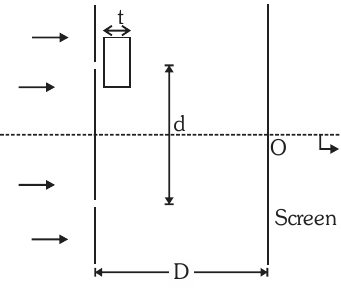
\includegraphics[width=0.5\linewidth]{Score-II - Test 02 (28 Mar 2021)-img/p2phy_q5_ydse.png}
\end{center}

\begin{qoptions}
\opt{A}{$\Delta\theta$ in terms of other given quantities is $\dfrac{(\mu-1)}{-(\mu-1)\alpha+\gamma}$}
\opt{B}{$\Delta\theta$ in terms of other given quantities is $\dfrac{(\mu-1)}{(\mu-1)\alpha+\gamma}$}
\opt{C}{If setup is placed in medium other than air, then $\Delta\theta$ will increase [If $\Delta\theta$ is positive]}
\opt{D}{If setup is placed in medium other than air, then $\Delta\theta$ will decrease [If $\Delta\theta$ is positive]}
\end{qoptions}

\textbf{6.} A circuit consists of a permanent source of e.m.f. E, a resistor R and a capacitor C connected in series. The internal resistance of the source is negligibly small. At the moment $t=0$, the capacitance of the capacitor was abruptly (jumpwise) decreased by a factor $\eta$. Then

\begin{center}
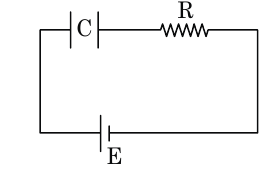
\includegraphics[width=0.4\linewidth]{Score-II - Test 02 (28 Mar 2021)-img/p2phy_q6_circuit.png}
\end{center}

\begin{qoptions}
\opt{A}{the current in the circuit as a function of time is $\dfrac{(\eta-1)E}{R}e^{-\eta t/RC}$}
\opt{B}{the current in the circuit as a function of time is $\dfrac{(\eta+1)E}{R}e^{-\eta t/RC}$}
\opt{C}{the current in the circuit just after the capacitance changes is $\dfrac{(\eta-1)E}{R}$}
\opt{D}{the current in the circuit just after the capacitance changes is $\dfrac{(\eta+1)E}{R}$}
\end{qoptions}

\textbf{7.} Consider two particles A and B of masses m and 2m at rest in an inertial frame. Each of them are acted upon by net forces of equal magnitudes F in the positive x-direction for equal amounts of time t. Momenta of the particles A and B in centre of mass frame are $\vec P_1$ and $\vec P_2$ respectively. Then

\begin{qoptions}
\opt{A}{$\vec P_1=\dfrac{F}{3}t\,\hat\imath$}
\opt{B}{$\vec P_1=\dfrac{2F}{3}t\,\hat\imath$}
\opt{C}{$\vec P_2=-\dfrac{F}{3}t\,\hat\imath$}
\opt{D}{$\vec P_2=-\dfrac{2F}{3}t\,\hat\imath$}
\end{qoptions}

\textbf{8.} For a glass prism the plot of deviation ($\delta$) vs angle of incidence (i) is as shown. If the refractive index of the glass is $\mu$ and value of angle is $i_1$. Then

\begin{center}
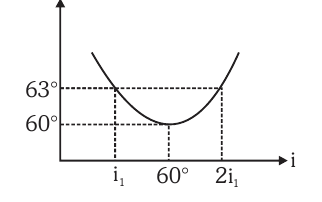
\includegraphics[width=0.45\linewidth]{Score-II - Test 02 (28 Mar 2021)-img/p2phy_q8_graph.png}
\end{center}

\begin{qoptions}
\opt{A}{$\mu=2$}
\opt{B}{$\mu=\sqrt3$}
\opt{C}{$i_1=30^\circ$}
\opt{D}{$i_1=41^\circ$}
\end{qoptions}

\subsectionhdr{Section-I (ii): List-Match}

\textbf{9--10.} A container of large uniform cross-sectional area A hold two immisible non-viscous and incompressible liquids of density d and 3d, each of height $\dfrac{H}{2}$. The lower density liquid is open to the atmosphere having pressure $P_0$. A tiny hole of area a ($a\ll A$) is punched on the vertical side of the lower container at a height $h\left[0<h<\dfrac H2\right]$ for which range `R' is maximum.

\begin{center}
\renewcommand{\arraystretch}{1.3}
\begin{tabular}{@{}p{0.62\linewidth}p{0.28\linewidth}@{}}
\textbf{List-I} & \textbf{List-II}\\
(I) h will be & (P) $\dfrac{2H}{3}$\\
(II) R will be & (Q) $\dfrac{H}{12}$\\
(III) V (velocity of efflux) will be & (R) $\sqrt{\dfrac{gH}{3}}$\\
(IV) Force on the vessel due to liquid flowing out will be & (S) $\dfrac72 dagH$\\
& (T) $2\,dagH$\\
& (U) None\\
\end{tabular}
\renewcommand{\arraystretch}{1.15}
\end{center}

\textbf{9.} If container is resting on the ground (horizontal surface), then:

\begin{center}
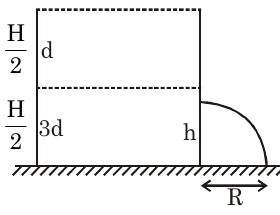
\includegraphics[width=0.28\linewidth]{Score-II - Test 02 (28 Mar 2021)-img/p2phy_q9_ground.png}
\end{center}

\begin{qoptions}
\opt{A}{I $\to$ P, II $\to$ Q, III $\to$ U, IV $\to$ U}
\opt{B}{I $\to$ Q, II $\to$ P, III $\to$ R, IV $\to$ T}
\opt{C}{I $\to$ U, II $\to$ P, III $\to$ U, IV $\to$ T}
\opt{D}{I $\to$ Q, II $\to$ P, III $\to$ R, IV $\to$ U}
\end{qoptions}

\textbf{10.} If container is placed on the top of table at height $\dfrac H2$, then:

\begin{center}
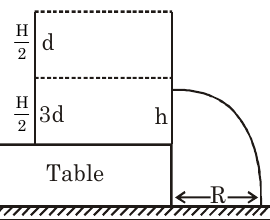
\includegraphics[width=0.38\linewidth]{Score-II - Test 02 (28 Mar 2021)-img/p2phy_q10_table.png}
\end{center}

\begin{qoptions}
\opt{A}{I $\to$ Q, II $\to$ U, III $\to$ U, IV $\to$ S}
\opt{B}{I $\to$ P, II $\to$ Q, III $\to$ U, IV $\to$ S}
\opt{C}{I $\to$ U, II $\to$ U, III $\to$ U, IV $\to$ U}
\opt{D}{I $\to$ Q, II $\to$ P, III $\to$ U, IV $\to$ U}
\end{qoptions}

\textbf{11--12.} A photo electric cell is shown in the figure. The emitter plate (cathode) is made of copper ($\phi=4.7$ eV) and emitter is illuminated by a source of monochromatic light of wavelength 200 nm. Saturation current is observed when potential difference between cathode and anode is 1V and anode at higher potential. [Range of ammeter is large] [Take hc $=1240$ (ev)nm]

\begin{center}
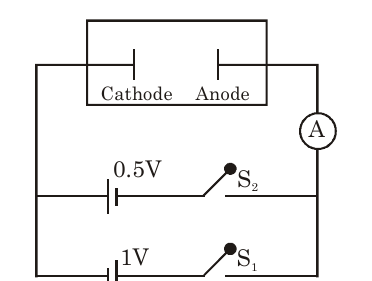
\includegraphics[width=0.55\linewidth]{Score-II - Test 02 (28 Mar 2021)-img/p2phy_q1112_circuit.png}
\end{center}

\begin{center}
\renewcommand{\arraystretch}{1.3}
\begin{tabular}{@{}p{0.62\linewidth}p{0.28\linewidth}@{}}
\textbf{List-I} & \textbf{List-II}\\
(I) Minimum kinetic energy of photoelectrons reaching the collector is & (P) 2.5 eV\\
(II) Maximum kinetic energy of photoelectrons reaching the collector is & (Q) Remain same\\
(III) If wavelength of incident light is decreased (no.\ of incident photon same), then reading of current as shown by ammeter will & (R) 1 eV\\
(IV) If number of incident photons increases, then reading of current as shown by ammeter will & (S) Increase\\
& (T) 0\\
& (U) Decrease\\
\end{tabular}
\renewcommand{\arraystretch}{1.15}
\end{center}

\textbf{11.} If only S$_1$ is closed, then:

\begin{qoptions}
\opt{A}{I $\to$ S, II $\to$ R, III $\to$ Q, IV $\to$ S}
\opt{B}{I $\to$ P, II $\to$ T, III $\to$ R, IV $\to$ S}
\opt{C}{I $\to$ T, II $\to$ P, III $\to$ S, IV $\to$ U}
\opt{D}{I $\to$ R, II $\to$ P, III $\to$ Q, IV $\to$ S}
\end{qoptions}

\textbf{12.} If only S$_2$ is closed, then:

\begin{qoptions}
\opt{A}{I $\to$ P, II $\to$ Q, III $\to$ S, IV $\to$ Q}
\opt{B}{I $\to$ T, II $\to$ R, III $\to$ Q, IV $\to$ S}
\opt{C}{I $\to$ S, II $\to$ T, III $\to$ P, IV $\to$ U}
\opt{D}{I $\to$ T, II $\to$ T, III $\to$ S, IV $\to$ Q}
\end{qoptions}

\subsectionhdr{Section-II: Numerical Value}

\textbf{1.} A point moves along a circle such that distance travelled $S=at^2$ [where $a=\dfrac12$ m/s$^2$] and t is time in second. Find the total acceleration of the point at the moment when it covered the $n^{\text{th}}$ ($n=0.10$) fraction of the circle after the beginning of the motion. [Take $\pi^2=10$]

\textbf{2.} A pulley block system inside lift is shown in figure. The pulleys and the threads are ideal and masses of the blocks are m and 5m. Find the minimum acceleration (in m/s$^2$) of the lift along vertically upwards direction for which the threads remain taut and both the blocks accelerate in the same direction relative to the ground. [Take $g=9.80$ m/s$^2$]

\begin{center}
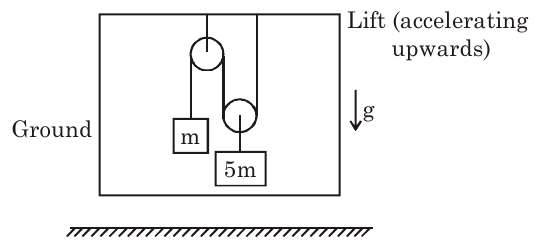
\includegraphics[width=0.55\linewidth]{Score-II - Test 02 (28 Mar 2021)-img/p2phy_n2_pulley.png}
\end{center}

\textbf{3.} 3 identical point particles of mass M move in such a way that distance between particles is `d' which remain constant. Only force is the gravitational force between particles. Then magnitude of relative velocity (in m/s) of one particle with respect to other particle will be:
\[\left[\text{Take}\ \sqrt{\dfrac{GM}{d}}=\sqrt3\ \text{m/s}\right]\]

\textbf{4.} A long, thin, pliable carpet is laid on the floor. One end of the carpet is bent back and then pulled backwards with constant unit velocity, just above the part of the carpet which is still at rest on the floor. What is the minimum force needed to pull the moving part, if the carpet has unit length and unit mass?

\begin{center}
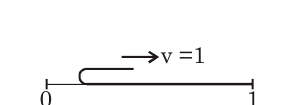
\includegraphics[width=0.4\linewidth]{Score-II - Test 02 (28 Mar 2021)-img/p2phy_n4_carpet.png}
\end{center}

\textbf{5.} Consider a uniformly charged solid cylinder of large length and radius R. Now consider a cylindrical surface of radius 2R and length 2R coaxial with cylinder and electric flux through cylindrical surface is $\phi_0$. Now consider a spherical surface of radius 2R and one of the diameter along axis of cylinder and electric flux through spherical surface is $\phi$. Find $\dfrac{\phi}{\phi_0}$.

\textbf{6.} A spherical bubble inside water has radius R. Take the pressure inside the bubble and the water pressure to be $P_0$. The bubble now gets compressed radially in an isothermal manner so that its radius become $(R-a)$. For $a\ll R$, the magnitude of work done in the process is given by $(4\pi P_0Ra^2)x$ where x is a constant. Find x.

\sectionhdr{PART-2: CHEMISTRY}
\subsectionhdr{Section-I (i): One or more correct}

\textbf{1.} Which of the following reagents is/are used for softening process of permanent hardness in water?

\begin{qoptions}
\opt{A}{Na$_6$P$_6$O$_{18}$}
\opt{B}{Na$_2$CO$_3$}
\opt{C}{Zeolite}
\opt{D}{Ca(OH)$_2$}
\end{qoptions}

\textbf{2.} IE$_1$ (kJ/mole) of $2^{\text{nd}}$ period elements are mentioned below with some blank/vacant data spaces:

\begin{center}
\renewcommand{\arraystretch}{1.2}
\begin{tabular}{cccccccc}
Li & Be & B & C & N & O & F & Ne\\
520 & ``P'' & 800 & ``Q'' & 1402 & 1314 & ``R'' & 2080\\
\end{tabular}
\renewcommand{\arraystretch}{1.15}
\end{center}

Select CORRECT number of statement(s) regarding above data table. (Consider all processes are gas phased).

\begin{qoptions}
\opt{A}{$|$EA$|$ of N$^+$ is more than 1402 kJ/mol}
\opt{B}{Value of ``R'' is more than 1402 kJ/mol}
\opt{C}{Value of ``P'' is more than $|$EA$|$ of C$^+$}
\opt{D}{Q $>$ 800 kJ/mol}
\end{qoptions}

\textbf{3.} In which reaction the product will react with 2,4-dinitrophenylhydrazine.

\begin{center}
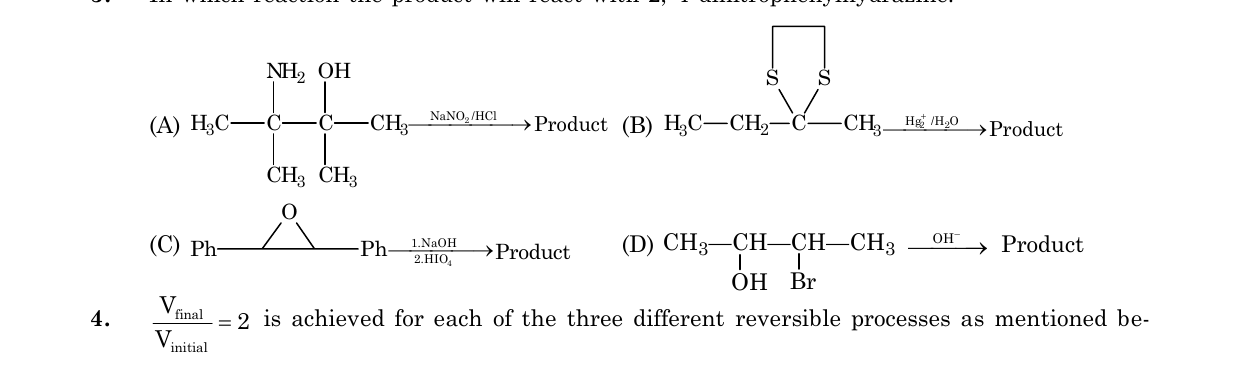
\includegraphics[width=0.95\linewidth]{Score-II - Test 02 (28 Mar 2021)-img/p2chem_q3_full.png}
\end{center}

\textbf{4.} $\dfrac{V_{\text{final}}}{V_{\text{initial}}}=2$ is achieved for each of the three different reversible processes as mentioned below. (1 mole of ideal gas with $\gamma=1.5$ for all processes)\\
(x) Isothermal process ending at state - A\\
(y) Isobaric process starting from state - A\\
(z) Reversible adiabatic process ending at state - B

\begin{center}
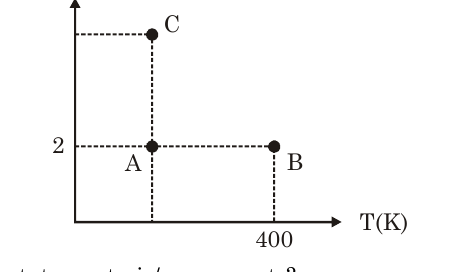
\includegraphics[width=0.5\linewidth]{Score-II - Test 02 (28 Mar 2021)-img/p2chem_q4_graph.png}
\end{center}

Which of the following statements is/are correct?

\begin{qoptions}
\opt{A}{Temperature of gas increases in two of the processes.}
\opt{B}{Maximum temperature observed during any of the processes is 400 K.}
\opt{C}{If ``C'' is initial state of isothermal process then $P_C=4$ atm.}
\opt{D}{Initial pressure of adiabatic process is more than initial pressure of isothermal process.}
\end{qoptions}

\textbf{5.} Intramolecular hydrogen bonding is NOT present in:

\begin{qoptions}
\opt{A}{crystalline orthoboric acid, B(OH)$_3$}
\opt{B}{Acetic acid in benzene solvent}
\opt{C}{crystals of ice}
\opt{D}{para-nitrophenol}
\end{qoptions}

\textbf{6.} Select correct options on basis of following seperation of reactions.

\begin{center}
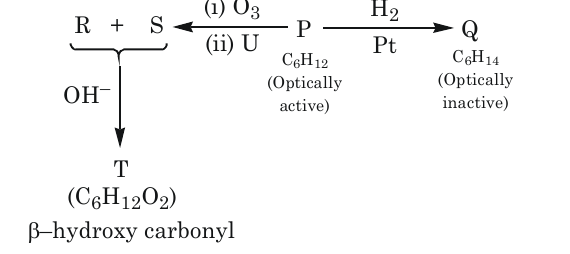
\includegraphics[width=0.75\linewidth]{Score-II - Test 02 (28 Mar 2021)-img/p2chem_q6_scheme.png}
\end{center}

\begin{qoptions}
\opt{A}{``Q'' does not have any 4$^\circ$ carbon.}
\opt{B}{Formation of T from ``R'' and ``S'' involve nucleophilic addition}
\opt{C}{``T'' compound is optically inactive.}
\opt{D}{Reagent ``U'' can be dimethyl sulphide.}
\end{qoptions}

\textbf{7.} Identify the incorrect statements when a fixed amount of ideal gas is heated in a container fitted with a movable piston always operating at constant pressure.

\begin{qoptions}
\opt{A}{Average distance travelled between successive collisions will decreases.}
\opt{B}{Collisions frequency increases since speed of the molecules increases with increases in temperature.}
\opt{C}{Average relative speed of approach remains unaffected.}
\opt{D}{Average angle of approach remains unaffected.}
\end{qoptions}

\textbf{8.} Choose the CORRECT statement(s) among the following.

\begin{qoptions}
\opt{A}{[Pd(Cl)$_4$]$^{2-}$ is tetrahedral geometry \& paramagnetic.}
\opt{B}{[Cr(NH$_3$)$_3$(Cl)$_3$] has 2 geometrical isomers \& 2 optical isomers.}
\opt{C}{[Co(H$_2$O)$_6$]$^{3+}$ is low spin while [CoF$_6$]$^{3-}$ is a high spin complex \& both cant show G.I.}
\opt{D}{[Fe(H$_2$O)$_5$(NO)]SO$_4$ has sp$^3$d$^2$ hybridisation and can't show optical isomers.}
\end{qoptions}

\subsectionhdr{Section-I (ii): List-Match}

\textbf{9--10.} Match the following.

\begin{center}
\renewcommand{\arraystretch}{1.25}
\begin{tabular}{@{}ll@{}}
\textbf{List-I} & \textbf{List-II}\\
(I) LiAlH$_4$ & (P) RCH=NOH\\
(II) NaBH$_4$ & (Q) RCOOH\\
(III) H$_2$/Pd & (R) R--CH=NH\\
(IV) B$_2$H$_6$ & (S) RCOCl\\
& (T) R--C$\equiv$N\\
& (U) R--CO--R\\
\end{tabular}
\renewcommand{\arraystretch}{1.15}
\end{center}

\textbf{9.} Which of the following combination is incorrect to produce amine.

\begin{qoptions}
\opt{A}{(II) - (R)}
\opt{B}{(I) - (P)}
\opt{C}{(III) - (T)}
\opt{D}{(II) - (S)}
\end{qoptions}

\textbf{10.} Which of the following combination is incorrect to produce alcohol.

\begin{qoptions}
\opt{A}{(III) - (U)}
\opt{B}{(II) - (S)}
\opt{C}{(IV) - (S)}
\opt{D}{(IV) - (Q)}
\end{qoptions}

\textbf{11--12.} Match the Matrix.

\begin{center}
\renewcommand{\arraystretch}{1.4}
\begin{tabular}{@{}p{0.5\linewidth}p{0.42\linewidth}@{}}
\textbf{List-I (Pairs of reaction)} & \textbf{List-II (Related observation in each pair of reaction)}\\
(I) Cr$^{3+}$(aq.) $\xrightarrow{\text{Excess Na}_2\text{O}_2}$ Product (X); \ Cr$^{3+}$(aq.) $\xrightarrow{\text{Excess Na}_2\text{O}}$ Product (Y) & (P) X is soluble but Y is precipitate\\
(II) Al$^{3+}$(aq.) $\xrightarrow{\text{Excess NaOH}}$ Product (X); \ Pb$^{2+}$(aq.) $\xrightarrow{\text{Excess NaOH}}$ Product (Y) & (Q) X and Y both are soluble\\
(III) S$^{2-}\xrightarrow{\text{BaCl}_2}$ Product (X); \ SO$_3^{2-}\xrightarrow[\text{H}_2\text{O}_2]{\text{BaCl}_2}$ Product (Y) & (R) Element X forms amphoteric oxide \& Y is a mixture of colourless gases\\
(IV) Electrolysis of molten Al$_2$O$_3$ along with Na$_3$AlF$_6$ \& CaF$_2$ giving X (at cathode) and Y (at anode) & (S) Y is soluble but X is precipitate\\
 & (T) X is yellow solution, Y is green solution\\
 & (U) X is a metal, Y is yellow gas\\
\end{tabular}
\renewcommand{\arraystretch}{1.15}
\end{center}

\textbf{11.} Which combination will give X \& Y as colourless solution.

\begin{qoptions}
\opt{A}{(I) - (T)}
\opt{B}{(II) - (Q)}
\opt{C}{(III) - (P)}
\opt{D}{(IV) - (U)}
\end{qoptions}

\textbf{12.} Select INCORRECT combination

\begin{qoptions}
\opt{A}{(I) - (T)}
\opt{B}{(III) - (S)}
\opt{C}{(I) - (Q)}
\opt{D}{(IV) - (R)}
\end{qoptions}

\subsectionhdr{Section-II: Numerical Value}

\textbf{1.} Silver ion forms a complex ion with thiosulphate ion, [Ag(S$_2$O$_3$)$_2$]$^{3-}$, with $K_f=2.8\times10^{13}$. How much AgBr ($K_{sp}=5.4\times10^{-13}$), in mole, will dissolve in 1 litre of 0.20 M Na$_2$S$_2$O$_3$ solution.

(Report your answer till two places after decimal) ($\sqrt{15.12}=3.88$)

\textbf{2.} Find $E_{\text{cell}}$ (volts) for
\[\resizebox{0.95\linewidth}{!}{$\text{Ag(s)} \mid \text{AgBr(s)} \mid \text{KBr(aq., }10^{-1}\text{M)} \,\|\, \text{KCl(aq., }10^{-6}\text{ M), AgCl(s)} \mid \text{Ag(s)}$}\]
Given, $K_{sp}$(AgCl) $=10^{-10}$ M$^2$. $K_{sp}$(AgBr) $=10^{-15}$ M$^2$.

\textbf{3.} Total number of compounds which are soluble in hot aqueous NaOH are:\\
(i) Salicyclic acid \hspace{1.5em} (ii) Aspirin\\
(iii) Formic acid \hspace{1.5em} (iv) Acetic acid\\
(v) Succinic anhydride \hspace{1.5em} (vi) Cyclohexanone\\
(vii) Benzene sulphonamide \hspace{1.5em} (viii) Cyclohexene

\textbf{4.} How many reaction enthalpy changes are marked incorrectly.\\
(i) CuSO$_4$(s) $+5$H$_2$O($\ell$) $\longrightarrow$ CuSO$_4\cdot5$H$_2$O(s) \ $(\Delta H_{\text{Solution}})_{\text{CuSO}_4(s)}$\\
(ii) 2NH$_3$(g) $\longrightarrow$ N$_2$(g) $+3$H$_2$(g) \ $(\Delta H^\circ_{\text{atomisation}})_{[\text{NH}_3(g)]}$\\
(iii) MgCl$_2$(s) $\longrightarrow$ Mg(g) $+2$Cl(g) \ $(\Delta H^\circ_{\text{lattice}})_{\text{MgCl}_2(g)}$\\
(iv) C(graphite) $+$O$_2$(g) $\longrightarrow$ CO$_2$(g) \ $(\Delta H^\circ_f)_{\text{CO}_2(g)}$\\
(v) N$_2$(g) $+3$H$_2$(g) $\longrightarrow$ 2NH$_3$(g) \ $(\Delta H^\circ_f)_{\text{NH}_3(g)}$

\textbf{5.} Consider the scheme below:

\begin{center}
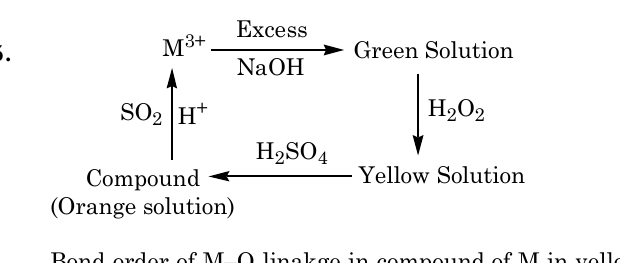
\includegraphics[width=0.5\linewidth]{Score-II - Test 02 (28 Mar 2021)-img/p2chem_sn5_scheme.png}
\end{center}

Bond order of M--O linkage in compound of M in yellow solution is \textbf{x}, number of M--O linkage in green solution compound is \textbf{y}, then value of (x $+$ y) is (M $=$ metal):

\textbf{6.} Predict the possible number of alkenes in the following reaction.

\begin{center}
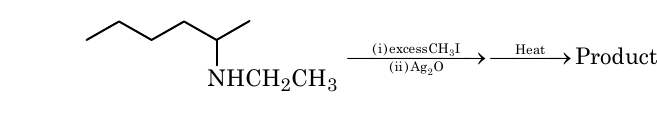
\includegraphics[width=0.6\linewidth]{Score-II - Test 02 (28 Mar 2021)-img/p2chem_sn6_structure.png}
\end{center}

\sectionhdr{PART-3: MATHEMATICS}
\subsectionhdr{Section-I (i): One or more correct}

\textbf{1.} If the centre of the arc represented by $\arg\left[\dfrac{(z-3i)}{(z-2i+4)}\right]=\dfrac{\pi}{4}$ is $\alpha+i\beta$, then

\begin{qoptions}
\opt{A}{$\beta=\dfrac92$}
\opt{B}{$\beta=\dfrac72$}
\opt{C}{$\alpha=\dfrac{-5}{4}$}
\opt{D}{$\alpha=\dfrac{-5}{2}$}
\end{qoptions}

\textbf{2.} There are three bags B$_1$, B$_2$ and B$_3$. The bag B$_1$ contains 4 red and 4 black marbles, B$_2$ contains 3 red and 4 black marbles, B$_3$ contains 4 red and 3 black marbles, Bags B$_1$, B$_2$ and B$_3$ have probabilities $\dfrac16,\dfrac13$ and $\dfrac12$ respectively of being chosen. A bag is selected at random and a marble is chosen at random from the bag. Then which of the following options is/are correct?

\begin{qoptions}
\opt{A}{Probability that the selected bag is B$_2$ and the chosen marble is black equals $\dfrac{4}{21}$.}
\opt{B}{Probability that chosen marble is red equals $\dfrac{43}{84}$.}
\opt{C}{Probability that chosen marble is red, given that selected bag is B$_1$ equals $\dfrac12$.}
\opt{D}{Probability that the selected bag is B$_2$ given that chosen marble is red equals $\dfrac{12}{43}$.}
\end{qoptions}

\textbf{3.} Two circles $x^2+y^2+2ax-c^2=0$ and $x^2+y^2+2bx-c^2=0$ meet in points P and Q. Parallel lines are drawn through P and Q to meet the circles in R and S as shown in figure. If locus of mid point of RS is $x^2+y^2+\lambda(a+b)x=0$, then the value of $\lambda$ is smaller than

\begin{center}
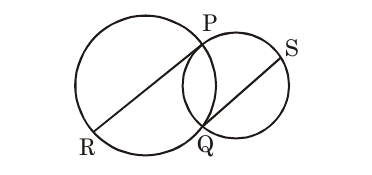
\includegraphics[width=0.4\linewidth]{Score-II - Test 02 (28 Mar 2021)-img/p2math_q3_circles.png}
\end{center}

\begin{qoptions}
\opt{A}{1}
\opt{B}{2}
\opt{C}{3}
\opt{D}{4}
\end{qoptions}

\textbf{4.} If matrix $A=\begin{pmatrix}a&b\\c&a\end{pmatrix}$ satisfies $A^{-1}=A$, then possible values of real number x such that $A-xI$ is not invertible is/are

\begin{qoptions}
\opt{A}{3}
\opt{B}{1}
\opt{C}{$-1$}
\opt{D}{4}
\end{qoptions}

\textbf{5.} If $f(x)=\begin{cases}|x|-3 & x<1\\ |x-2|+a & x\ge1\end{cases}$ and $g(x)=\begin{cases}2-|x| & x<2\\ \operatorname{sgn}(x)-b & x\ge2\end{cases}$

and $h(x)=f(x)+g(x)$ is continuous $\forall\, x\in\mathbb{R}$ then which of the following options is/are incorrect

\begin{qoptions}
\opt{A}{Value of `a $-$ b' is 4}
\opt{B}{Value of `a $-$ b' is $-3$}
\opt{C}{Value of `a $+$ b' is 2}
\opt{D}{Value of `a $+$ b' is $-2$}
\end{qoptions}

\textbf{6.} The value of
\[\resizebox{0.95\linewidth}{!}{$\displaystyle\lim_{x\to\frac{\pi}{2}}\left(12\tan^2x\left(\sqrt{6+3\sin x-2\cos^2x}-\sqrt{3+6\sin x-\cos^2x}\right)\right)$}\]
is less than:

\begin{qoptions}
\opt{A}{0}
\opt{B}{1}
\opt{C}{2}
\opt{D}{3}
\end{qoptions}

\textbf{7.} Let $b\in\mathbb{R}-\{0\}$, suppose $f:\mathbb{R}\to\mathbb{R}^+$ is a differentiable function such that $f(0)=1$. If the derivative $f'$ of f satisfies the equation $f'(x)=\dfrac{f(x)}{\sqrt{b^2-x^2}}$ for all $x\in\mathbb{R}$, then which of the following statements is/are true?

\begin{qoptions}
\opt{A}{Monotonic behaviour of $f(x)$ depends on b.}
\opt{B}{Monotonic behaviour of $f(x)$ is independent of b.}
\opt{C}{$f(x)\cdot f(-x)=1$ for $x\in(-b,b)$}
\opt{D}{$f(x)\cdot f(-x)=-1$ for $x\in(-b,b)$}
\end{qoptions}

\textbf{8.} A normal to the hyperbola $\dfrac{x^2}{4}-\dfrac{y^2}{1}=1$ at point P in Ist quadrant has equal intercepts on the positive x and y-axis at point A and B respectively. The tangent at point `P' cut x-axis at point C. The normal at point `P' also touches the ellipse $\dfrac{x^2}{a^2}+\dfrac{y^2}{b^2}=1$. If $\Delta_1=$ Area of $\triangle PAC$ and $\Delta_2=$ area of $\triangle PBC$, then

\begin{qoptions}
\opt{A}{The value of $a^2+b^2$ is $\dfrac{25}{3}$}
\opt{B}{The value of $a^2+b^2$ is $\dfrac{50}{3}$}
\opt{C}{$\dfrac{\Delta_1}{\Delta_2}=\dfrac14$}
\opt{D}{$\dfrac{\Delta_1}{\Delta_1}=\dfrac{1}{\sqrt2}$}
\end{qoptions}

\subsectionhdr{Section-I (ii): List-Match}

\textbf{9--10.} Given the continuous function
\[y=f(x)=\begin{cases}x^2+10x+8 & x\le-2\\ ax^2+bx+c & -2<x<0,\ a\ne0\\ x^2+2x & x\ge0\end{cases}\]
Line L touches the graph of $y=f(x)$ at 3 points. There are some expression given in the List-I whose values are given in List-II below:

\begin{center}
\renewcommand{\arraystretch}{1.25}
\begin{tabular}{@{}ll@{}}
\textbf{List-I} & \textbf{List-II}\\
(I) Slope of line L is & (P) 2\\
(II) The value of a $+$ b $+$ c is & (Q) 3\\
(III) The value of $a^2+b-c$ is & (R) 4\\
(IV) The value of $a\times b-c$ is & (S) 5\\
& (T) 6\\
& (U) 7\\
\end{tabular}
\renewcommand{\arraystretch}{1.15}
\end{center}

\textbf{9.} Which of the following is only correct combination.

\begin{qoptions}
\opt{A}{(I)$\to$(P)}
\opt{B}{(I)$\to$(Q)}
\opt{C}{(II)$\to$(U)}
\opt{D}{(II)$\to$(T)}
\end{qoptions}

\textbf{10.} Which of the following is only Incorrect combination.

\begin{qoptions}
\opt{A}{(I)$\to$(R)}
\opt{B}{(III)$\to$(Q)}
\opt{C}{(III)$\to$(U)}
\opt{D}{(IV)$\to$(T)}
\end{qoptions}

\textbf{11--12.} Consider a triangular pyramid ABCD, the position vectors of whose angular points are A(3, 0, 1), B($-1$, 4, 1), C(5, 2, 3) and D(0, $-5$, 4). Let G be the point of intersection of the medians of triangle BCD. There are some expression given in the List-I whose values are given in List-II below:

\begin{center}
\renewcommand{\arraystretch}{1.3}
\begin{tabular}{@{}p{0.62\linewidth}p{0.28\linewidth}@{}}
\textbf{List-I} & \textbf{List-II}\\
(I) The length of vector $\overrightarrow{AG}$ is & (P) $\dfrac{14}{\sqrt6}$\\
(II) Area of $\triangle ABC$ is & (Q) $\dfrac{4}{\sqrt6}$\\
(III) Length of perpendicular from vertex D on opposite face is & (R) $4\sqrt6$\\
(IV) Area of $\triangle ABD$ is & (S) $\dfrac{\sqrt{51}}{3}$\\
& (T) $2\sqrt{82}$\\
& (U) $\sqrt{82}$\\
\end{tabular}
\renewcommand{\arraystretch}{1.15}
\end{center}

\textbf{11.} Which of the following is the only correct combination:

\begin{qoptions}
\opt{A}{(I)$\to$(S)}
\opt{B}{(III)$\to$(Q)}
\opt{C}{(IV)$\to$(R)}
\opt{D}{(IV)$\to$(Q)}
\end{qoptions}

\textbf{12.} Which of the following is only Incorrect combination:

\begin{qoptions}
\opt{A}{(IV)$\to$(T)}
\opt{B}{(II)$\to$(R)}
\opt{C}{(III)$\to$(P)}
\opt{D}{(II)$\to$(P)}
\end{qoptions}

\subsectionhdr{Section-II: Numerical Value}

\textbf{1.} A sports person wants to practice for exactly 5 days during coming 20 days, but he doesn't want to tire himself. So he decided to have at least 2 days of rest between two practice sessions. Find the no of ways in which he can do so.

\textbf{2.} Total number of onto functions $f:\{1,2,3,4,5\}\to\{3,4,5,6,7\}$ such that $f(i)\ne i+2$ is

\textbf{3.} Two fair dice are rolled together and the sum of the numbers on the faces is observed. If p is the probability of getting sum as prime number before the sum is obtained as perfect square, then the value of 88p.

\textbf{4.} Let $d_n$ be the distance travelled by the fighter plane in $n^{\text{th}}$ hour. $d_{n+1}=2d_n+n(1+2^n)$, $\forall\, n=1,2,3,4,\ldots$ where $d_1=1$. If $d_n=(n^2-2n+13)2^{n-2}-(n+1)$ for some particular n, then value of n is:

\textbf{5.} $\displaystyle\int_{-3}^{3} x^{16}\left\{x^{17}\right\}dx$ is equal to $\dfrac{3^\lambda}{\mu}$. ($\{.\}$ is fractional part) then the smallest value of $\lambda+\mu$ is equal to (where $\lambda,\mu\in\mathbb{N}$)

\textbf{6.} If x $+$ 4y is a normal to the curve $y^2=\alpha x^3-\beta$ at (2, 3), then the value of $\alpha+\beta$ is

\end{document}
